\subsection{Generic Programming, \CC\ and Templates}

\cgal\ is a \CC\ library and follows in its design the \emph{generic
programming paradigm\/}~\cite{cgal:ms-aogl-94,cgal:sl-stl-95} and in
a few places also design patterns~\cite{Gamma:1995:DP}. Generic
programming has found wide spread acceptance in the \CC\ community
with the \emph{Standard Template Library}, \stl, as its prominent
example as part of the \CC\ Standard Library. The good \stl\ 
introduction and reference book~\cite{cgal:a-gps-98} coins the terms
\emph{concept} for a set of requirements imposed on a template
parameter, and \emph{model\/} for all types that fulfill the set of
requirements and can thus be used as template argument. An example
function template:
\begin{lstlisting}
template <typename T>
void swap( T& a, T& b) { T tmp = a; a = b; b = tmp; }
\end{lstlisting}
This generic \CodeFmt{swap} function requires from the template
parameter \CodeFmt{T} to have a copy constructor and an assignment
operator. This is collectively summarized under the \emph{concept\/}
\textsc{Assignable}. Now, each builtin type, such as \CodeFmt{double},
has a copy constructor and assignment operator and thus is a
\emph{model\/} of \textsc{Assignable}. In the \stl , concepts are
defined for container classes, iterators that link container classes
with algorithms, function objects that are an efficient and type safe
generalization of function pointers, allocators, and many more. In
particular iterators are interesting for us. They represent
abstractions of pointers. Several concepts are defined for iterators,
depending on their capability of traversing the underlying sequence of
elements in a container class, i.e., input and output iterator for
simple read once or write once sequences, forward iterator for single
linked lists, bidirectional iterator for doubly-linked lists, and
random-access iterator for array-like data structures. More recent
textbooks introducing template programming techniques
are~\cite{Alexandrescu:2001:MCD,cgal:vj-ctcg-03}.

\subsection{Computational Geometry Algorithms Library}

The development of \cgal, the Computational Geometry Algorithms
Library, started in 1995 and the first public release appeared in June
1997. \cgal\ is since its release 3.0 in November 2003 an Open Source
project initiated by a consortium of European and Israelean research
institutes with the goal to
\begin{quote}
    {\em make the large body of geometric algorithms developed in the field
    of computational geometry available for industrial application.}
\end{quote}
\cgal's main design goals are correctness, flexibility, efficiency,
and ease of use. Its focus is on a broad foundation in computational
geometry. Important related issues, for example visualization, are
supported with standard formats and interfaces.

An overview of \cgal\ is given in~\cite{Kettner04Handbook}. The design
is thoroughly covered in~\cite{fgkss-dccga-00} and generic programming
aspects are discussed in~\cite{bksv-agppd-00}. \cgal\ is roughly
structured into a geometric kernel and a basic library. The geometric
kernel contains the geometric primitives, such as points, vectors,
triangles, and predicates and constructions on those geometric
primitives, and has an extendible design described
in~\cite{hhkps-aegk-01}. 

The basic library contains data structure and
algorithms.  Their design follows the \stl\ design with iterator based
interfaces, etc. The basic library is decoupled from the geometric
primitives, i.e., there exists a template parameter in each
algorithm and data structure of the basic library that represents the
connection to the geometric primitives, predicates, and constructions.
For suitable subsets we define concepts, for example,
that are sufficient to run the two-dimensional convex hull algorithms,
and call them the \emph{geometric traits concept for two-dimensional
convex hull}. For many geometric traits classes, a \cgal\ geometric
kernel is a valid model.

There are many choices for a \cgal\ geometric kernel. One can choose
between reference counted and non-reference counted storage, between
Cartesian or homogeneous coordinate
representation\footnote{Homogeneous coordinates are only used to have
  efficient implementations of exact integer arithmetic without
  divisions, and not for projective geometry. \cgal\ works in affine
  geometry.}, and the number type used to store coordinates and do the
arithmetic. The right choice for the number type is essential for the
correctness of some of the algorithms and data structures. The main
distinction in \cgal\ is along the boundary of exact predicate
evaluation and exact construction of new primitives. Exact predicate
evaluation can be done efficiently with clever filtering
techniques~\cite{bbp-iayed-01} while point coordinates can be stored
efficiently in the conventional \CodeFmt{float} or \CodeFmt{double}
value. On the other hand, exact constructions needs a more powerful
number type in the geometric primitive coefficients that can also
represent newly constructed geometric primitives exactly. This means
usually exact long integer arithmetic. 
%We see an example below.

\subsection{Edge-based Mesh Data Structures}

The first reported edge-based mesh data structures are the
winged-edge~\cite{Baumgart:1975:PRCV} and the doubly-connected edge
list (DCEL)~\cite{Muller78}. Both store one data record per edge and
even simple traversals in the mesh neighborhood needed case
distinctions. The key inside was the split of the edge into two
halfedges~\cite{Weiler85,Maentylae88} (also referred to as DCEL
nowadays), which allows to encode orientation in the mesh and
traversal simplifies to mere pointer traversal. The edge
split can be done in two ways, either assigning a halfedge to each
incident facets, or assigning a halfedge to each incident
vertex~\cite{Weiler85}, these are duals of each other. Thinking of
both splits at once leads to the quad-edge data 
structure~\cite{Guibas:1983:PMG} that, deploying an additional bit per
quad-edge and per referring pointer, can also represent non-orientable
2-manifold surfaces. A detailed comparison of these structures can be
found in~\cite{k-ugpdd-99}.

Halfedge data structures (and similarly quad-edge) have been very
successful for the design of algorithms on meshes for several reasons:
\begin{itemize}
\item halfedges have a constant number of adjacencies. 
\item halfedges encode the mesh orientation.
\item navigation around vertices or facets is easy.
\item corner attributes, such as crease normals, can be associated
      with halfedges.
\end{itemize}


\subsection{Generic Mesh Data Structures}

The quad-edge data structure is the theoretically most appealing data
structure, however, non-orientable surfaces are typically not of interest in
mesh algorithms, and the strict symmetry between vertices and facets
makes this structure troublesome in a strong typed system where
vertices and facets are different types. Getting the asymmetry back
leads to the halfedge data structure in \cgal, where a halfedge is 
associated with a facet (see Fig.\ref{fig:halfedge}). The details
of the halfedge data structure and the \cgalpoly\ based on it are
described in~\cite{k-ugpdd-99}. We review the necessary parts in the
following sections.

\begin{figure}[htb]
    \centering{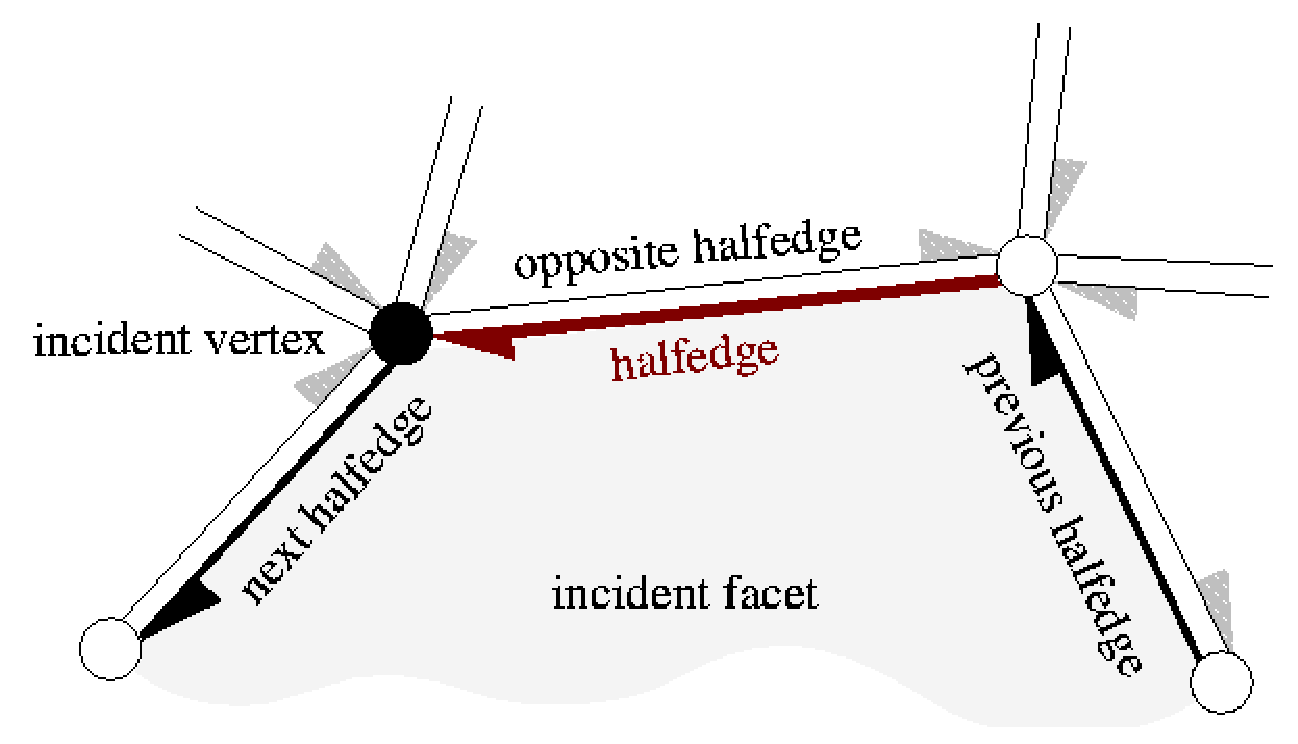
\includegraphics[width=5.0cm]{figs/halfedge}}
    \caption{One halfedge and its incident primitives. The next
      halfedge, the opposite halfedge, and the incident vertex are
      mandatory, the remaining elements are optional and can be
      selected by the user.}
    \label{fig:halfedge}
\end{figure}

Starting from the design described in~\cite{k-ugpdd-99}, a thorough
analysis of the potential design space of such an edge-based data
structure was given in~\cite{cgal:b-digph-01}. This analysis pointed
out some design choices that are not realizable in the design of
\cgalpoly. For example, although an array (\CodeFmt{std::vector}) can
be used to store the mesh elements, a reference to elements must
always be a pointer or iterator, and cannot be an index into that
error.

The same observation led the developers in the \openmesh\ 
project, see Release 1.0.0-beta4 at \path|http://www.openmesh.org/|,
to modify the \cgal\ design for their mesh data structure. Among
others does their design allow indices instead of pointers, and they
have a specialized data structure for meshes that consist only of
triangles~\cite{Botsch:2002:OPENMESH}. This redesign comes at a price
in readability of the user code; while the design of \cgalpoly\ allows
the direct traversal from item to item, i.e., direct expressions such
as
\begin{lstlisting}
facet_handle->halfedge()->opposite()->facet()
\end{lstlisting}
are possible, while in \openmesh\ the choice of an index always
requires the knowledge of the data structure itself, and potentially
more costly array arithmetic to access an item, such as in the
equivalent example now written for \openmesh
\begin{lstlisting}
hds.face_handle(
    hds.opposite_halfedge_handle(
        hds.halfedge_handle(facet_handle))).
\end{lstlisting}
The obvious question is, does it matter, and if, for which design. We
have a first answer in favior for the more readable \cgal\ design with
a runtime comparison of the $\sqrt{3}$ subdivision algorithm in
Section~\ref{sec:sqrt3}. However, this is only one application used
for comparison and the result should be taken with a grain of salt.
Both solutions are quite flexible and complex. Different applications
and maybe tests on individual operations would be needed for a more
conclusive answer. 














% % Related work and background

% % C++ and generic programming
% \noindent \textbf{CGAL and generic programming paradigm.}
% Before using CGAL, it is mandatory to be familiar with C++,
% \emph{design patterns} and the \emph{generic programming paradigm}. 
% Design patterns \cite{Gamma:1995:DP} describe successful and
% \emph{reusable} solutions to standard software problems. The generic
% programming paradigm \cite{Alexandrescu:2001:MCD} features the notion
% of C++ class templates and function templates, which is at the corner
% stone of all features provided by CGAL. 

% The generic programming paradigm provides a
% soft-coupled framework to support data structures and algorithms. 
% It focuses on representing families of the data structures 
% or the algorithms by identifying 
% the \emph{abstract representations}.
% With the \CC\ template, the standard template library
% \cite{ms-stl-96} (STL) is the pioneer library based on
% the generic programming paradigm. The STL provides a set of 
% data structure families (or containers), such as vectors, 
% lists and trees, and a set of generic algorithms 
% that can be dynamicly coupled with a container. In general, 
% the abstract representation of a data structure family
% is the \emph{entity type} and of an algorithm family
% is the \emph{operation type}. 
% %For example are the entity sorting and searching where users
% %supply the equality predicates to specialize the algorithms.  
% To soft couple the containers and the algorithms, STL 
% use the \italic{iterator} concept to be the interface.
% An iterator allows both referring to an enitity (as a \CC\ pointer) 
% and visiting a sequence of entities in the container.
% The STL frees software engineers from rebuilding the fundamental 
% data structures and let them focus on the design of the algorithms.
% Since CGAL is strongly inspired
% from the generality of STL, it is important to become familiar with
% its concepts before starting using it.

% \noindent \textbf{Geometry data structures.}
% A polyhedral mesh consists the adjacency relationships
% among a set of primitives, i.e.\ vertices, edges and 
% facets. A polyhedron data structure describes 
% the adjacency relationships and the storage of the
% primitives. Several different data structures
% of polyhedral meshes are proposed in the past.
% Most prominent of them are the so-called
% edge-based data structures 
% \cite{Weiler:1985:EDS,Baumgart:1975:PRCV,Guibas:1983:PMG}.
% Edge-based data structures highlight the
% adjacency relationships among the edges
% and link the incidental vertices and facets
% by the stored pointers. Edge-based data structures
% are commonly used and allow for maximal flexibility.
% Among them, the \emph{halfedge data structure} is the most
% commonly used. 

% \input hds

% OpenMesh \cite{Botsch:2002:OPENMESH} is ...

%\noindent \textbf{Geometry algorithms.}
% % Subdivision surfaces \cite{cc,ds,loop,sqrt3,qts}
% % is the limit surface resulted from the
% % application of a subdivision algorithm to a control polyhedron.
% % Subdivision algorithms recursively \emph{refine} (subdivide) the
% % control polyhedron and \emph{modify} (smooth) the geometry according
% % to the stencils of the source mesh.  
%Subdivisions consist of two
%meta-steps that most geometry processing algorithms have: the
%\emph{connectivity operation} and the
%\emph{geometry operation}. In this paper, we use subdivision
%as the template of the geometry processing algorithms because it
%connectivity operations are more complex than most other
%algorithms. Some other simple algorithms, e.g.\ displacement map, the
%connectivity operation is a null operation. In other words, the source
%and the target mesh have the same connectivity.

%Further details on subdivisions can be found at \cite{Sub:course:2000}
%and \cite{Warren:subdivision}. The OpenMesh library has
%supports of Loop and $\sqrt{3}$ subdivisions \cite{Abhijit:2004:APISUB}.
